
\documentclass[a4paper]{article}

\usepackage{url}
\usepackage{amsmath}
\usepackage{verbatim}   		% Useful for program listings
\usepackage[T1]{fontenc}       	% For Swedish characters ÅÄÖ etc.
\usepackage[utf8]{inputenc}
% \usepackage[swedish]{babel} % For Swedish hyphenation
\usepackage{fancyvrb}           	% For lists with tabulators
\fvset{tabsize=4}              	 	% Tabulator size
\fvset{fontsize=\small}         	% List font size
\usepackage{graphicx}		% Imports the graphicx package, useful for images

% generate clickable references & toc
\usepackage[]{hyperref}
\hypersetup{
%    pdftitle={Your title here},
%    pdfauthor={Your name here},
%    pdfsubject={Your subject here},
%    pdfkeywords={keyword1, keyword2},
    bookmarksnumbered=true,
    bookmarksopen=true,
    bookmarksopenlevel=1,
    colorlinks=true,
    pdfstartview=Fit,
    pdfpagemode=UseOutlines,    % this is the option you were lookin for
    pdfpagelayout=TwoPageRight
}

% define namedlabel as per http://texblog.org/2012/03/21/cross-referencing-list-items/
% this is used for naming the requirements.
\usepackage{enumitem, hyperref}
\usepackage{nameref}



%% Macros for mapping
% - use case to subsection level
% - scenario to subsubsection level
% - requirement to paragraph level
%
% Using these results in it being possible to cross-reference
% requirements and getting unique identifiers which are author-chosen.

% usage: \usecase{cross-reference}{display-reference} text text ...
\newcommand{\usecase}[2]{
  \subsection*{#2}
  \label{#1}
  \addcontentsline{toc}{subsection}{\nameref{#1}}
}


% usage: \scenario{cross-reference}{display-reference} text text ...
\newcommand{\scenario}[2]{
  \subsubsection*{#2}
  \label{#1}
  \addcontentsline{toc}{subsubsection}{\nameref{#1}}
}

 % usage: \requirement{cross-reference}{display-reference} text text ...
\newcommand{\requirement}[2]{
  \paragraph*{#2:}
  \label{#1}
  \addcontentsline{toc}{paragraph}{\nameref{#1}}
}




\title{Dragonfly Quadrotor UAV \\ System Requirements Specification}
\author{Eduardo Riffo \\ Abed Shoka}

\date{\today}
%\date{December, 2015}         		% Today's date if not specified


\begin{document}                	% Start of document

\maketitle                      	% Prints the title defined above with \title, \author and \date

\begin{center}
\vspace{64pt}

\includegraphics[scale=1.6]{images/AF_Logotype20141_Black.png}
\vspace{16pt}
\\ \large ÅF Technology
\end{center}

\vspace{16pt}
\begin{tabular}{ l l l p{8.5cm} }
	Ver. & Date & Name & Description and Reason for change \\\hline
	0.1 Draft & December 14, 2015 & Eduardo & Created document structure.\\
\end{tabular}

\begin{table}[]
\centering
\caption{Document approval}
\begin{tabular}{c c c c}
\hline\hline
Signature & Name & Title & Date \\ [0.5ex]
\hline
	& & & \\
	& & & \\
	& & & \\
\hline
\end{tabular}
\label{table:nonline}
\end{table}

\newpage

\tableofcontents				% Insert table of contents

\newpage

\section{Introduction}

The System Requirement Specification (SRS) document is a technical description of the functional and non-functional requirements needed for the Dragonfly project. A system design picture containing the Dragonfly system and all its subsystem is described below. This document should contain all of the information needed by a software engineer to adequately design and implement the software product described by the requirements listed in this document.

\begin{figure}[!h]
	\centering
	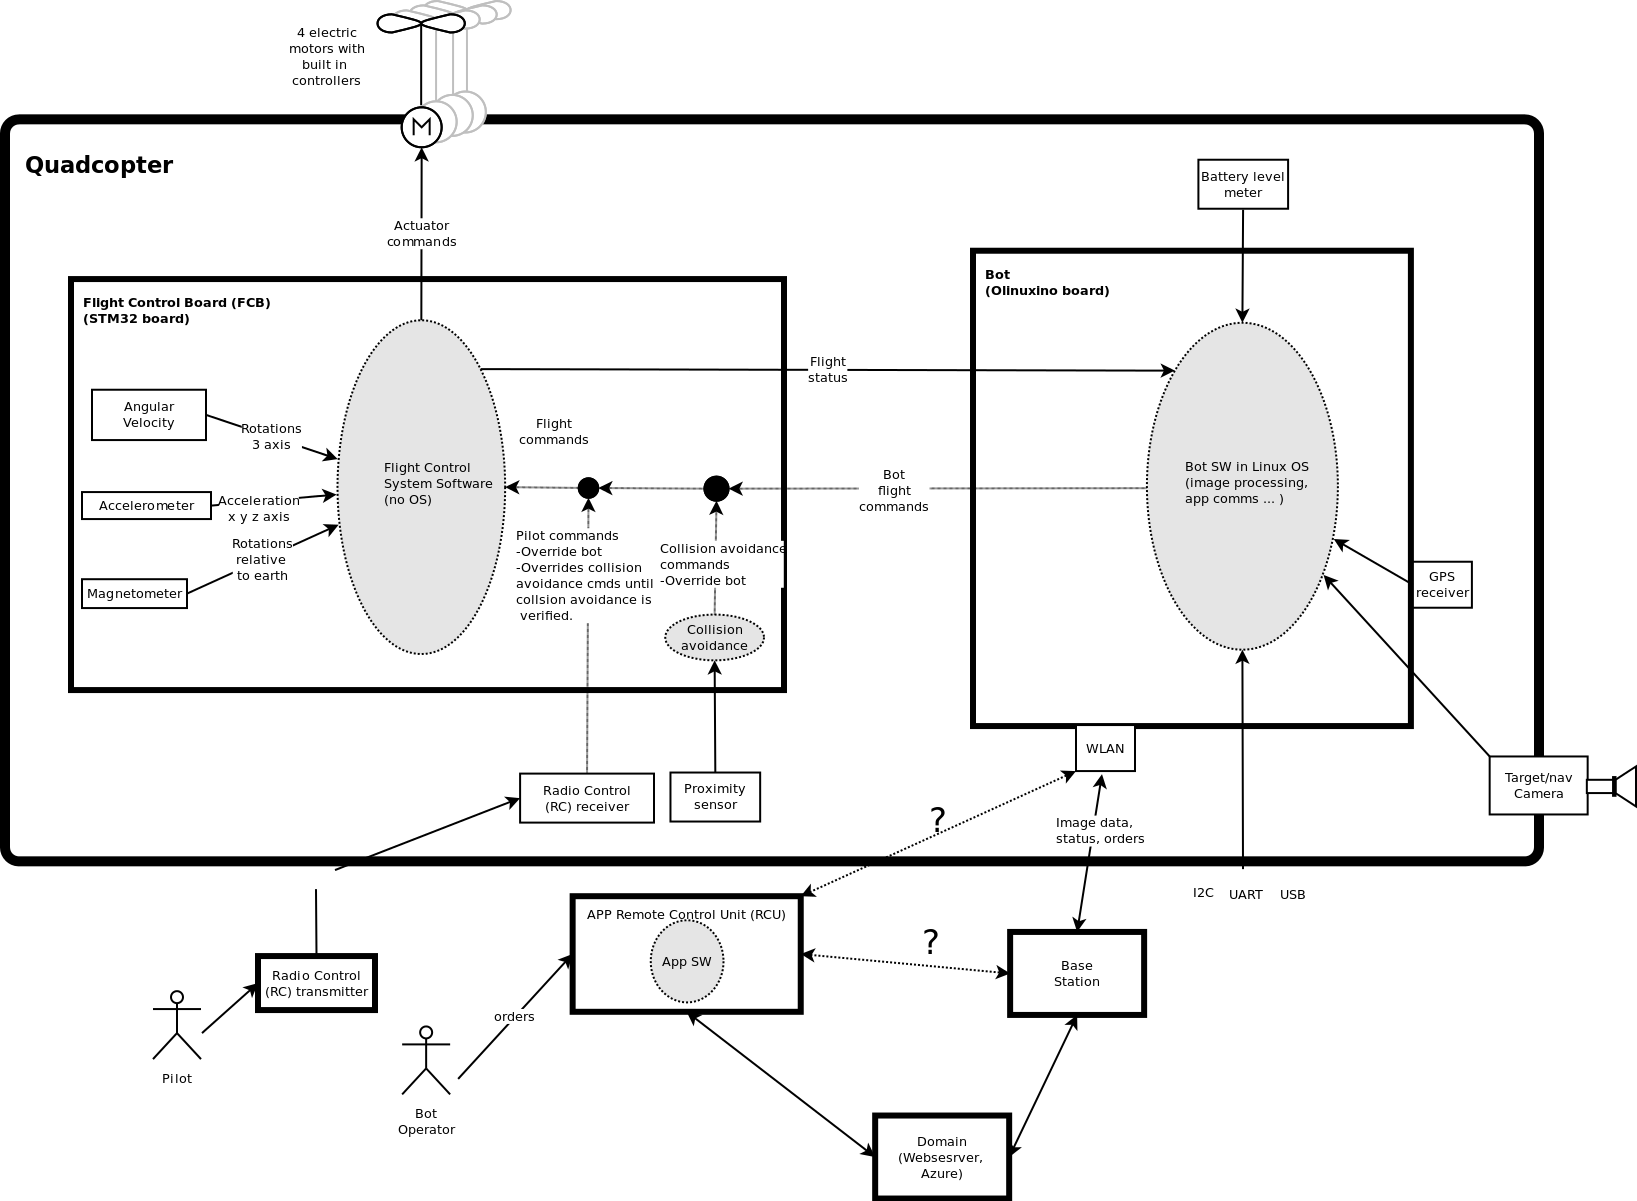
\includegraphics[width=\textwidth]{images/SystemArchitectureDiagram_DF.png}
	\caption{SystemArchitectureDiagram}
	\label{fig:sysarchdiag}
\end{figure}

\subsection{Purpose}

The purpose of this SRS is to list all the system requirements and how they map to PRS requirements and use cases. The intended audience is of this document are all involved in the dragonfly project.

\subsection{Scope}

The subsystems that are part of the dragonfly system is:
\begin{itemize}
	\item Charger subsystem. Which is responsible for controlling charge level and charging the Dragonfly UAV Quadcopter unit. It will also suggest or redirect to an available charging base.
	By doing so it enables optimised usage of the dragonfly from a charging point of view.
	\item subsystem X.
	\item Subsystem Y.
\end{itemize}

\subsection{Definition, Acronyms and Abbreviations}

The SRS contains the following definitions of terms, acronyms, and abbreviations required to properly interpret the SRS.
\begin{itemize}
	\item SRS - System Requirement Specification.
	\item PRS - Product Requirement Specification.
	\item UC  - Use case definition.
\end{itemize}

\subsection{References}

\begin{thebibliography}{99}
	\bibitem{Dragonfly-PRS} Dragonfly Product Requirement Specification, 2015
	\bibitem{Dragonfly-UC} Dragonfly Use Case Description, 2015
\end{thebibliography}

\subsection{Overview}

\section{General Description}

The SRS describes the general factors that affect the dragonfly project and its requirements on the different subsystem. It should be made clear that this section does not state specific requirements; it only makes those requirements easier to understand.

\subsection{Product Perspective}

This subsection of the SRS puts the dragonfly product into perspective with other related products requirements or projects goals.

\subsection{Product Functions}

The summary of the product requirements are listed in \cite{Dragonfly-PRS}.


\subsection{General Constraints}

This SRS only describes the dragonfly and charger base as product entity, all other components that are a considered  a part of the either the dragonfly or the charger base.
From a software point of view all sub-system are considered to be a part of the dragonfly system.

\subsection{Assumptions and Dependencies}

This part of the SRS list each of the factors that affect the requirements stated in the SRS. These factors are not design constraints on the software but are, rather, any changes to them that can affect the requirements in the SRS.
It is assumed that the flight control board (FCB) runs a freeRTOS and has an interface to the flight management system (FMS) that will run on a Linux debian armhfs distribution. All the different hardware components should interface either the FMS or the FCB and be controlled by its corresponding subsystem.

\section{Specific Requirements}

This section is the largest and most important section of the SRS.

Each requirement in this section should be:
\begin{itemize}
\item	Correct
\item	Traceable (both forward and backward to prior/future artifacts)
\item	Unambiguous
\item	Verifiable (i.e., testable)
\item	Prioritised (with respect to importance and/or stability)
\item	Complete
\item	Consistent
\item	Uniquely identifiable (usually via numbering like 3.4.5.6)
\end{itemize}
Note that this SRS is not a software design document, therefore one should avoid the tendency to over-constrain and design the software project within this SRS.

\subsection{External Interface Requirements}
\requirement{req:PRS-CH002}{PRS-CH002}: The Quadcopter receiver and transmitter must be placed within a fixed distance.
\requirement{req:PRS-CH013}{PRS-CH013}: Charging base should be covered by plastic glass with a predetermined thickness.

\subsubsection{User Interfaces}
\subsubsection{Hardware Interfaces}
\subsubsection{Software Interfaces}
\subsubsection{Communications Interfaces}

\subsection{External Interface Requirements}
\requirement{req:PRS-CH005}{PRS-CH005}: Charging base must enable power supply manually User interaction is mandatory for this process, since it involves tweaking the voltage.
\subsubsection{User Interfaces}
\subsubsection{Hardware Interfaces}
\subsubsection{Software Interfaces}
\subsubsection{Communications Interfaces}

\subsection{External Interface Requirements}
\requirement{req:PRS-CH006}{PRS-CH006}: Enable balanced server charger manually.
\subsubsection{User Interfaces}
\subsubsection{Hardware Interfaces}
\subsubsection{Software Interfaces}
\subsubsection{Communications Interfaces}

\subsection{Functional Requirements}

\subsubsection{Functional Requirement SRS-CH001}
\requirement{req:SRS-CH001}{SRS-CH001}: The Quadcopter unit must have receiver coil attached to receiver cuircuit and a balanced server charger. Complies with {SRS-CH001}.
\paragraph{Introductions}
\paragraph{Inputs}
\paragraph{Processing}
\paragraph{Outputs}
\paragraph{Error Handling}

\subsubsection{Functional Requirement SRS-CH001}
\requirement{req:PRS-CH003}{PRS-CH003}: The Quadcopter unit must implement a software based capacity monitor.
\paragraph{Introductions}
\paragraph{Inputs}
\paragraph{Processing}
\paragraph{Outputs}
\paragraph{Error Handling}

\subsubsection{Functional Requirement SRS-CH001}
\requirement{req:PRS-CH003}{PRS-CH003}: The Quadcopter unit must implement a software based capacity monitor.
\paragraph{Introductions}
\paragraph{Inputs}
\paragraph{Processing}
\paragraph{Outputs}
\paragraph{Error Handling}

\subsubsection{Functional Requirement SRS-CH001}
\requirement{req:PRS-CH007}{PRS-CH007}: Investigate if Inductive changer used in project can be controlled automatically  through software.
\paragraph{Introductions}
\paragraph{Inputs}
\paragraph{Processing}
\paragraph{Outputs}
\paragraph{Error Handling}

\subsubsection{Functional Requirement SRS-CH001}
\requirement{req:PRS-CH008}{PRS-CH008}: Motion sensors needs to be enabled to guaranty effective charging.
\paragraph{Introductions}
\paragraph{Inputs}
\paragraph{Processing}
\paragraph{Outputs}
\paragraph{Error Handling}

\subsubsection{Functional Requirement SRS-CH001}
\requirement{req:PRS-CH009}{PRS-CH009}: Mechanism to turn the power supply off should be implement if possible. Monitoring of charging process must be done to avoid overheating and unnecessary  power consumption.
\paragraph{Introductions}
\paragraph{Inputs}
\paragraph{Processing}
\paragraph{Outputs}
\paragraph{Error Handling}

\subsubsection{Functional Requirement SRS-CH001}
\requirement{req:PRS-CH010}{PRS-CH010}: Charging notifications must be implemented and sent to users or quadcopter unit.
\paragraph{Introductions}
\paragraph{Inputs}
\paragraph{Processing}
\paragraph{Outputs}
\paragraph{Error Handling}

\subsubsection{Functional Requirement SRS-CH001}
\requirement{req:PRS-CH011}{PRS-CH011}: Suggest the nearest charging base to user, but let the user make decision.
\paragraph{Introductions}
\paragraph{Inputs}
\paragraph{Processing}
\paragraph{Outputs}
\paragraph{Error Handling}

\subsubsection{Functional Requirement SRS-CH001}
\requirement{req:PRS-CH012}{PRS-CH012}: Automatic charging redirection to charging base must be supported by Quadcopter unit.
\paragraph{Introductions}
\paragraph{Inputs}
\paragraph{Processing}
\paragraph{Outputs}
\paragraph{Error Handling}



\subsection{Use Cases}
All use cases used by the different subsections or use case referrals are listed in \cite{Dragonfly-UC}.

\subsection{Classes / Objects}
All classes, objects, functions and attributes for addressing functional requirements are to be solved by their corresponding user story. See corresponding user story description in the project.

\subsection{Non-Functional Requirements}
Non-functional requirements for the dragonfly system will be listed in this sub chapter.

\subsubsection{Performance}
The dragonfly performance must be robust and FMS system be thread-safe, meaning if a thread hangs it must be possible to restart it without affecting the whole dragonfly system.
\paragraph{Reliability}
Navigation and orientation must be reliable constantly, if a sensor needed for navigation is malfunctioning or is broken, the Dragonfly quadcopter unit must land in a controlled manner.
\paragraph{Security}
Due to the size and weight of the Dragonfly quadcopter unit, it is crucial that the flight management has a recovery mode if something happens to main dragonfly system. If the FMS is unresponsive it is up the FCB to perform a smooth and controlled landing, ensuring that neither the quad copter unit nor other object can be harmed or destroyed.
\paragraph{Maintainability}
The system software of the Dragonfly quadcopter unit may only be updated and/or upgraded during development and stabilization phase of the project. After executing the corresponding user story and meeting definition of "Done", upgrade and update should not be performed.

\subsection{Design Constraints}
There Dragonfly has hardware constraints, due to weight limitation and charging capacity. All components that needs to be added, has to be evaluated with these constraints.

\subsection{Other Requirements}
Other requirements that are not covered by the Dragonfly System Design are NOT covered by this SRS.

\section{Analysis Models}
All analysis models used in developing specific functional requirements are covered by its corresponding user story.  See corresponding userstory for more information.. Traceability will be tracked in the user story document.

\end{document}                  % End of document
